\chapter{Laufzeitsicht}
In diesem Kapitel werden die Abläufe zwischen den Controllern erklärt. Es wird auf die Teile der Controller-Kommunikation eingegangen, 
die einer expliziten Erläuterung bedürfen.
\section{Select}

\begin{figure}[htb!]
	\caption{Select Sequenzdiagramm}
	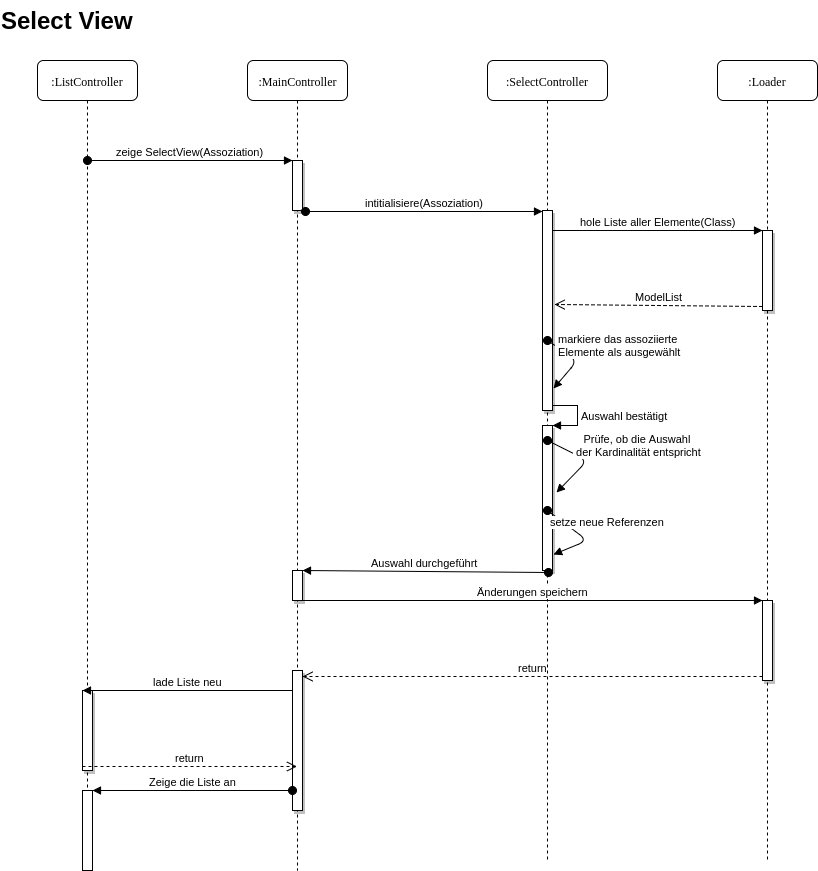
\includegraphics[width=0.9\textwidth]{content/pictures/SelectSeq}
	\label{pic:selectSeq_diag}
\end{figure}

Die Select Funktionalität wird von der Listenasicht zur Verfügung gestellt. Sie wird nur für die Assoziationsdarstellung benötigt. 
Der Ablauf ist in dem Diagramm \ref{pic:selectSeq_diag} dargestellt. Zu vermerken ist, dass die Validerung der Auswahl anhand der
Kordinalität seiner Assoziation, nicht unter die Aufgaben des SelectViewControllers fällt.  

\section{ShowList}

\begin{figure}[htb!]
	\caption{ShowList Sequenzdiagramm}
	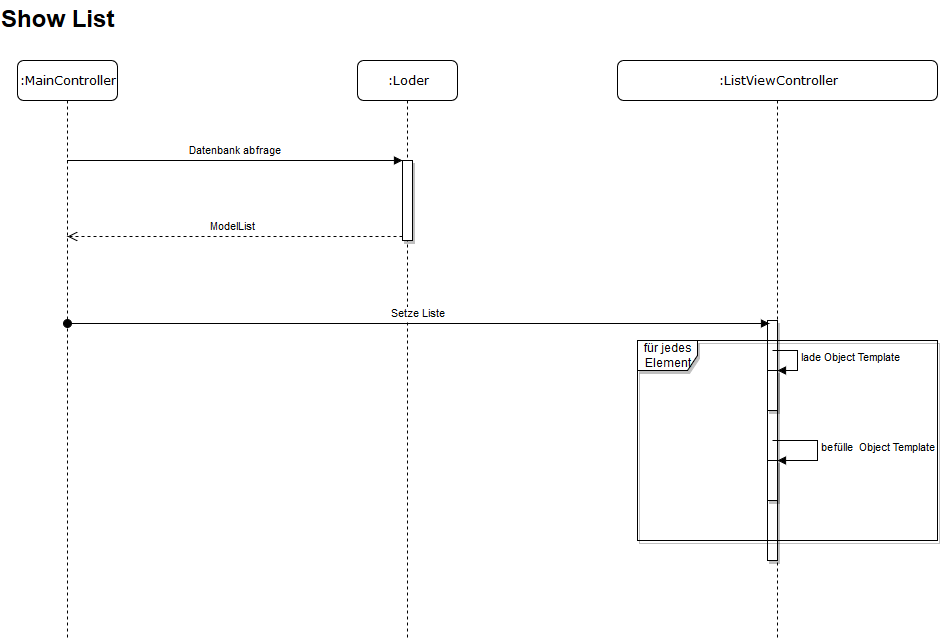
\includegraphics[width=0.9\textwidth]{content/pictures/ShowListSeq}
	\label{pic:showListSeq_diag}
\end{figure}

Der Ablauf bei der Erstellung der Listenansicht ist in dem Diagramm \ref{pic:showListSeq_diag} dargestellt. Dabei bindet 
das ListView-Template zugehörige Objekt-Templates zur Laufzeit ein. Die Datenobjekte und die Information, ob der Nutzer
die Daten bearbeiten darf, werden bei der Anbindung übergeben. Eine Typprüfung der Datenobjekte findet nicht statt.

\section{CreateNewView}

Das Diagramm \ref{pic:createNewViewSeq_diag} stellt die Kommunikation zwischen den Controller-Elementen bei der Erstellung eines neun
Datenobjekts dar. Der Vorgang kann aus der ListView ausgelöst werden. Der Ablauf unterscheidet sich abhängig davon, ob es sich bei
dem Ausgangselement um eine \enquote{ModelList} oder \enquote{Association} handelt. Bei einer Association kann das Datenobjekt automatisch bei der Erstellung gestzt
werden.

\begin{figure}[H]
	\caption{CreateNewView Sequenzdiagramm}
	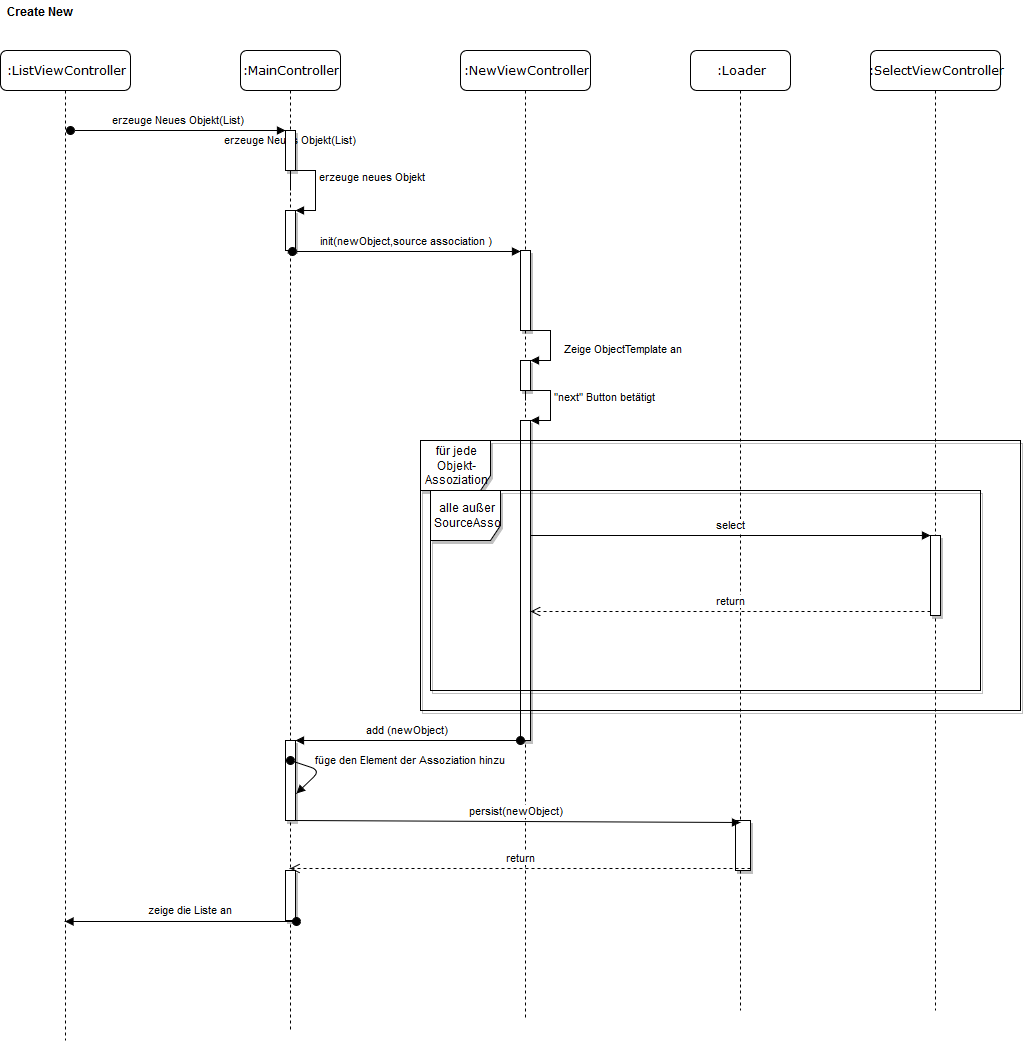
\includegraphics[width=0.9\textwidth]{content/pictures/CreateNewView}
	\label{pic:createNewViewSeq_diag}
\end{figure}

